\documentclass[../thesis.tex]{subfiles}
\graphicspath{{../gfx/}{gfx/}}
\begin{document}

\pagestyle{plain}
\chapter{Wprowadzenie teoretyczne}

Celem tego rozdziału jest dostarczenie opisu podstawowych zagadnień związanych z uczeniem maszynowym. W szczególności rozdział ten poświęcony jest dwóm dziedzinom wiedzy: przetwarzaniu wstępnemu oraz (późniejszej) klasyfikacji danych. Końcowa część rozdziału poświęcona jest testom statystycznym, a szczególnie testowi Manna-Whitneya-Wilcoxona.

\section{Klasyfikacja}

Klasyfikacja statystyczna to rodzaj algorytmu, który przydziela obserwacje statystyczne do klas, bazując na atrybutach tych obserwacji \cite{def_classification}. Algorytm klasyfikacji tworzy model klasyfikacji na podstawie danych trenujących zawierających znane klasy (kategorie). Gotowy model można następnie zastosować  do predykcji kategorii nowych, nieznanych wcześniej, obserwacji. Klasyfikacja jest zatem przykładem uczenia się z nadzorem. Nadzór polega na obecności w zbiorze trenującym informacji o kategoriach danych, które mamy. Algorytm tworzenia modelu stara się nauczyć model docelowych kategorii, jednocześnie dbając o to, aby wiedza na temat problemu była jak najbardziej ogólna i niezależna od próby, którą dysponujemy.

\begin{figure}[h]
\centering
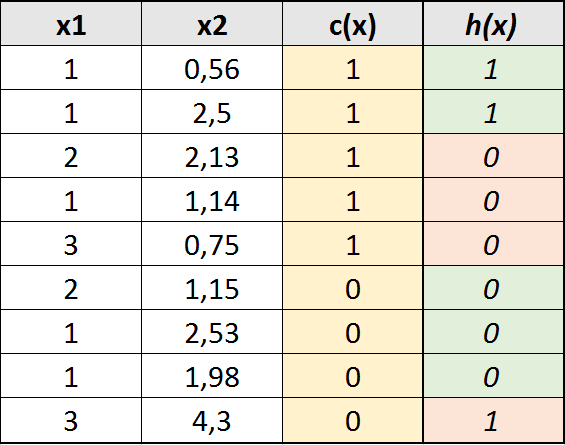
\includegraphics[height=.2\textheight]{classification.png}
\caption{Przykład klasyfikacji danych o atrybutach \emph{x\textsubscript{1}}, \emph{x\textsubscript{2}} oraz kategorii \emph{c(x)}. Kolumna \emph{h(x)} oznacza hipotezę klasyfikatora (predykcję). Dwa pierwsze przykłady zostały zaklasyfikowane poprawnie, trzy następnie niepoprawnie, następne trzy poprawnie, a ostatni nieprawidłowo. }
\label{classification:basic}
\end{figure}

\subsection{Ocena klasyfikacji}

W celu oceny gotowego modelu klasyfikacji, możemy posłużyć się miarami zdefiniowanymi na podstawie zawartości tzw. macierzy pomyłek. Dla klasyfikacji dwuwartościowej macierz pomyłek składa się z dwóch wierszy i dwóch kolumn. Kolumny odpowiadają faktycznym kategoriom danych, wiersze zaś predykcjom klasyfikatora. Na przecięciu kolumn i wierszy znajdują się cztery wartości liczbowe charakteryzujące poprawność wyników modelu. Wartości \emph{True Positive} i \emph{True Negative} określają ile poprawnych wyników pozytywnych i negatywnych zostało zwróconych przez klasyfikator. Z kolei wartości \emph{False Positive} i \emph{False Negative} pokazują, ile pozytywnych i negatywnych przypadków model zaklasyfikował niewłaściwie.

\begin{figure}[h]
\centering
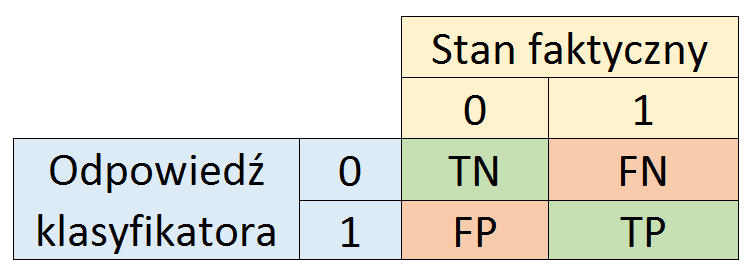
\includegraphics[height=.1\textheight]{error_matrix.png}
\caption{Przykładowa macierz pomyłek.}
\label{classification:error_matrix}
\end{figure}

Ocenę jakości modelu klasyfikacji łatwo wyrazić wartościami liczbowymi wyliczanymi w oparciu na poszczególnych komórkach macierzy pomyłek. Celnością $c$ nazywamy stosunek liczby poprawnych wyników klasyfikacji do wszystkich rozpatrywanych przypadków:
\[c = \frac{t_p + t_n}{t_p + t_n + f_p + f_n}\]
gdzie $t_p$, $t_n$, $f_p$ i $f_n$ oznaczają odpowiednio wartości \emph{True Positive}, \emph{True Negative}, \emph{False Positive} i \emph{False Negative}. Miara ta pokazuje, jak często klasyfikator daje poprawny wynik. W medycynie częściej jednak stosuje się inne miary oceny, w szczególności \emph{precyzję} i \emph{wrażliwość}. 

Precyzja odpowiada na pytanie, jaka część zdiagnozowanych przypadków była prawdziwa. Precyzję $p$ wyrażamy jako stosunek liczby poprawnie zdiagnozowanych przypadków do liczby wszystkich pozytywnych wyników predykcji modelu:
\[p = \frac{t_p}{t_p + f_p}\]
gdzie $t_p$ i $f_p$ oznaczają odpowiednio wartości \emph{True Positive} i \emph{False Positive}.

Druga miara - wrażliwość - pokazuje nam, jaka część chorych została wykryta przez klasyfikator. Wrażliwość $w$ wyraża się jako iloraz liczby słusznie zdiagnozowanych przypadków oraz liczby wszystkich zachorowań:
\[w = \frac{t_p}{t_p + f_n}\]
gdzie $t_p$ i $f_n$ oznaczają odpowiednio wartości \emph{True Positive} i \emph{False Negative}.

W praktyce trudno jednak o model, który ma jednocześnie wysokie wartości precyzji i wrażliwości. Z tego powodu często stosuje się miarę \emph{F1}, będącą średnią harmoniczną dwóch powyższych miar:
\[f_1 = \frac{2t_p}{2t_p + f_p + f_n}\]
gdzie $f_1$, $t_p$, $f_p$ i $f_n$ to odpowiednio wartość miary \emph{F1}, a następnie wartości \emph{True Positive}, \emph{False Positive} i \emph{False Negative}.

\subsection{Nadmierne dopasowanie}

Oceniając jakość klasyfikacji nie należy zapominać o problemie nadmiernego dopasowania modelu. Nadmierne dopasowanie to zjawisko zachodzące, gdy model klasyfikacji daje gorsze wyniki dla nowych danych niż dla znanych danych trenujących. Aby ocena modelu nie była obarczona błędem związanym z tym zjawiskiem, do ewaluacji klasyfikatora należy używać osobnego zbioru testowego rozłącznego ze zbiorem trenującym.

\begin{figure}[h]
\centering
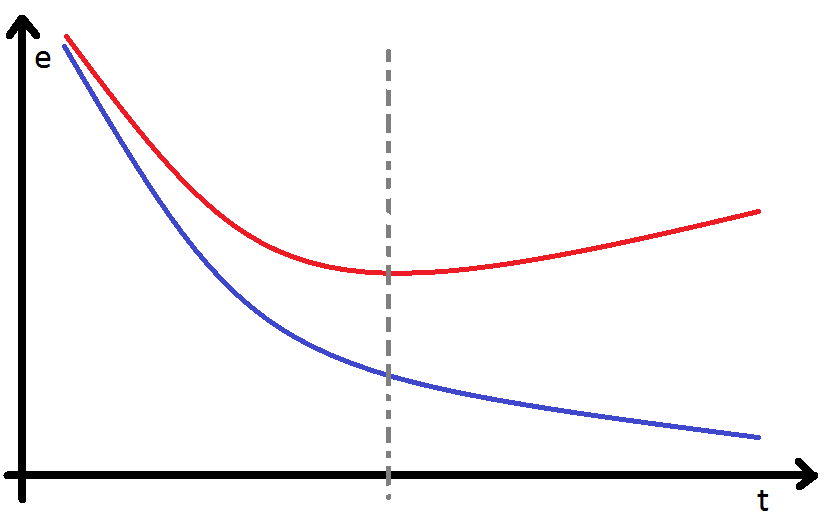
\includegraphics[height=.2\textheight]{overfitting.png}
\caption{Wykresy zależności błędu klasyfikatora od czasu związanego z nauką. Linia niebieska prezentuje błąd na zbiorze trenującym, który nieprzerwanie maleje z czasem. Wykres czerwony przedstawia błąd rzeczywisty na całej populacji danych. Nadmierne dopasowanie zaczyna się od momentu zaznaczonego szarą linią - błąd rzeczywisty zaczyna rosnąć.}
\label{classification:overfitting}
\end{figure}

Dzieląc dostępne dane na zbiór trenujący i testowy należy pamiętać o konsekwencjach tego podziału. Im mniejszy jest zbiór uczący (a testowy większy) tym mniej informacji stosujemy do nauki modelu i końcowa ocena może być zaniżona. Z drugiej strony, im mniejszy jest zbiór testowy, tym mniej jest reprezentatywny dla całej populacji i tym większa będzie wariancja oceny na tym zbiorze. 

Z  powyższym problemem można radzić sobie wykonując wiele testów. W literaturze wyróżnia się zwykle dwie metody z tym związane: \emph{sprawdzian krzyżowy} (inaczej: walidacja krzyżowa) oraz \emph{metoda bootstrap}.

Sprawdzian krzyżowy polega na podziale danych na $n$ równolicznych części, utworzeniu danych uczących z $n-1$ z nich i przeprowadzeniu testów na pozostałej części. Uczenie i ocenę modelu powtarza się $n$-krotnie, za każdym razem dla innych części. Otrzymane $n$ ocen można użyć np. do wyliczenia oceny końcowej, będącej średnią. 

Metoda bootstrap tworzy zbiór uczący poprzez losowanie ze zwracaniem ze zbioru danych wejściowych. Przykłady niewylosowane stają się zbiorem testowym.

\subsection{Przegląd algorytmów klasyfikacji}

Do najpopularniejszych klasyfikatorów stosowanych obecnie należą naiwny klasyfikator bayesowski, drzewo decyzyjne, las losowy oraz maszyna wektorów nośnych. Dalsza część rozdziału skupi się na omówieniu tych algorytmów.

\subsubsection{Naiwny klasyfikator bayesowski}

Naiwny klasyfikator bayesowski jest klasyfikatorem probabilistycznym. Oznacza to, że dla danego przykładu wynikiem zwracanym przez model są prawdopodobieństwa poszczególnych kategorii. Klasyfikator ten znany jest od ponad 60 lat – badania nad nim prowadzone były już w latach 50 XX w. Zasada działania tego klasyfikatora opiera się na twierdzeniu Bayesa, znanym z probabilistyki:
\[P(c_i|x) = \frac{P(c_i)P(x|c_i)}{P(x)}\]
gdzie $P(c_i|x)$ oznacza prawdopodobieństwo, że przykład $x$ należy do kategorii $c_i$, $P(c_i)$ oznacza prawdopodobieństwo wystąpienia kategorii $c_i$ w ogóle, $P(x|c_i)$ to prawdopodobieństwo wystąpienia przykładu $x$ pod warunkiem zaistnienia kategorii $c_i$, a $P(x)$ to prawdopodobieństwo wystąpienia przykładu $x$.

Naiwność tej metody klasyfikacji polega na założeniu, że wewnątrz kategorii, atrybuty są względem siebie niezależne. W wielu przypadkach założenie to nie jest spełnione, co odbija się na jakości oceny klasyfikatora. Mimo tej oczywistej wady, naiwny klasyfikator bayesowski znajduje praktyczne zastosowanie, np. przy diagnozowaniu niektórych chorób.

\subsubsection{Drzewo decyzyjne}

Kolejny popularnym klasyfikatorem jest drzewo decyzyjne. W trakcie uczenia modelu budowane jest drzewo, w którego węzłach znajdują się testy na wartości atrybutów, a w liściach kategorie lub prawdopodobieństwa kategorii. W trakcie predykcji przykład wędruje od korzenia drzewa do liścia, przechodząc konkretnymi gałęziami w zależności od wyników testów w węzłach. Popularność drzewa decyzyjnego bierze się m.in. z tego, że bardzo często daje ono zadowalające wyniki klasyfikacji. 

Częstym problemem drzew decyzyjnych jest duży rozrost wgłąb i, towarzyszące temu, nadmierne dopasowanie do danych trenujących. Z problemem tym można walczyć, przycinając drzewo, tj. zastępując poddrzewa liśćmi. Postępowanie takie wynika z przekonania, że modele mniej skomplikowane lepiej generalizują wiedzę. Wśród algorytmów przycinania wyróżnia się m.in.: \emph{Reduced Error Pruning}, \emph{Minimum Error Pruning} oraz \emph{Cost Complexity Pruning}.

\subsubsection{Las losowy}

Rozwinięciem pomysłu związanego z drzewami decyzyjnymi jest klasyfikator znany jako las losowy (ang. \emph{random forest}). Klasyfikator ten to zbiór drzew decyzyjnych, z których każde nauczone jest na oddzielnym zbiorze trenującym uzyskanym \emph{metodą boostrap}. Podczas predykcji przykład przechodzi przez każde z drzew, generując przy tym serię wyników. Rezultaty tych pomniejszych klasyfikacji grupowane są w zbiorowy ranking, na podstawie którego klasyfikator losowy las podejmuje ostateczną decyzję co do kategorii przykładu.

\begin{figure}[h]
\centering
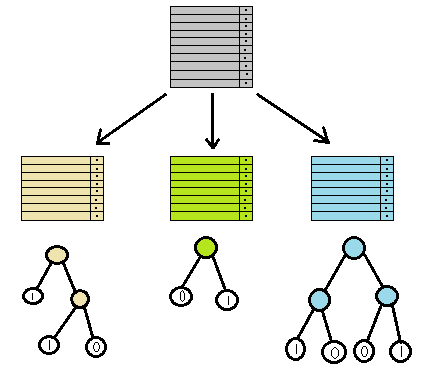
\includegraphics[height=.3\textheight]{random_forest.png}
\caption{Poglądowa ilustracja przedstawiająca las losowy składający się z trzech drzew decyzyjnych.}
\label{classification:random_forest}
\end{figure}

\subsubsection{Maszyna wektorów nośnych}

Ostatnim klasyfikatorem omówionym w tej części pracy jest Maszyna Wektorów Nośnych. Jest to klasyfikator binarny. Nauka modelu klasyfikatora ma na celu wyznaczenie hiperpłaszczyzny rozdzielającej z maksymalnym marginesem przykłady należące do dwóch klas.

\section{Przetwarzanie wstępne}

Celem przetwarzania wstępnego, w kontekście uczenia maszynowego i klasyfikacji, jest zamiana oryginalnej postaci danych wejściowych na taką, która umożliwia uzyskiwanie lepszych wyników późniejszej klasyfikacji \cite{def_preprocessing}. W mojej pracy dyplomowej korzystam z pewnych metod wstępnego przetwarzania danych i badam ich wpływ na końcową ocenę klasyfikacji. W części tej omawiam użyte przeze mnie metody, jak również kilka innych.

\subsection{Transformacje danych}

\subsubsection{Standaryzacja}

Wiele algorytmów klasyfikacji oczekuje wartości atrybutów o rozkładzie przypominającym standardowy rozkład normalny. Dane, którymi dysponujemy, mogą być zgrupowane w innej postaci. Aby zapewnić dobre wyniki klasyfikacji, często stosuje się \emph{standaryzację}. Metoda ta polega na przesunięciu danych o ich wartość średnią w kierunku zera i późniejszym podzieleniu przez wartość odchylenia standardowego:
\[x_i^{std} = \frac{x_i - \mu(X)}{\sigma(X)}\]
gdzie $x_i^{std}$ oznacza nową wartość po standaryzacji, $x_i$ wartość początkową, $\mu(X)$ wartość średnią atrybutu, a $\sigma(X)$ odchylenie standardowe atrybutu. Po wykonaniu powyższej operacji rozkład danych przypomina standardowy rozkład normalny.

\subsubsection{Skalowanie}

Innym rozwiązaniem jest \emph{skalowanie} atrybutów. Polega ono na proporcjonalnym przeskalowaniu wartości atrybutu tak, aby znalazły się w ustalonym przedziale. Częstymi docelowymi przedziałami są [0, 1] i [-1, 1]. Przekształcenie opisuje następująca zależność:
\[x_i = r_s + (r_e - r_s)\frac{x_i - X_{min}}{X_{max} - X_{min}}\]
gdzie $x_i$ oznacza nową wartość atrybutu po przeskalowaniu, $r_s$ początek docelowego przedziału, $r_e$ koniec docelowego przedziału, $X_{min}$ minimalną wartość atrybutu, a $X_{max}$ wartość maksymalną.

\begin{figure}[h]
\centering
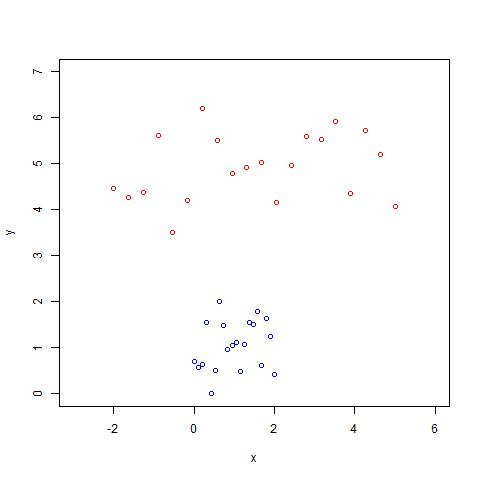
\includegraphics[height=.4\textheight]{scale.jpg}
\caption{Dane oryginale przed skalowaniem (czerwone punkty) oraz po przeskalowaniu do zakresu [0, 2] w osiach \emph{X} i \emph{Y} (niebieskie punkty).}
\label{classification:scale}
\end{figure}

\subsubsection{Normalizacja}

Metoda \emph{normalizacji} stanowi inne spojrzenie na modyfikowanie danych. Zamiast działać na atrybutach, normalizacja zajmuje się pojedynczymi przykładami z danych. Metoda ta polega na takim przeskalowaniu przykładu, aby jego długość (rozumiana w sensie interpretacji wektorowej) była równa 1. W praktyce oznacza to podzielenie wektora przykładu przez jego normę:
\[\vec{x_n} = \frac{\vec{x}}{\|\vec{x}\|}\]
gdzie $\vec{x_n}$ oznacza przykład znormalizowany, $\vec{x}$ przykład początkowy, a $\|\vec{x}\|$ normę wektora (przykładu).

\subsubsection{Binaryzacja}

Przedstawione do tej pory metody koncentrowały się na skalowaniu danych. W odróżnieniu od nich, \emph{binaryzacja} polega na zamianie wartości atrybutów na zera i jedynki. Wybór pomiędzy dwoma liczbami  opiera się na wartości ustalonego progu. Wszystkie wartości atrybutów większe od progu zamieniane są na jedynki, pozostałe zaś – na zera. Po zastosowaniu binaryzacji każdy przykład stanowi pewną kombinację zer lub jedynek. Pozwala to nam interpretować przykłady jako realizacje schematu Bernoulliego, gdzie jedynka oznacza sukces, a zero porażkę.

\subsection{Brakujące wartości atrybutów}

Cztery metody opisane w poprzednim punkcie zakładają, że wśród danych nie ma brakujących wartości. W realnych zastosowaniach często niestety jest inaczej – dane, którymi dysponujemy, mają  pewien odsetek braków. Przykładowo, dane medyczne użyte w mojej pracy mają 8\% brakujących wartości. Nawet, jeżeli przyjmiemy, że wyżej wymienionych metod nie będzie się stosować, to wciąż niektóre algorytmy klasyfikacji wymagają kompletnych danych. Wyróżniamy zwykle dwie metody rozwiązywania tego problemu.

\subsubsection{Usuwanie przykładów}

Pierwszą z metod jest usuwanie przykładów, w których występują braki, i dalsza praca na pełnych danych. Jest to najprostsza metoda, ale również posiadająca pewne niepożądane konsekwencje. Po pierwsze, eliminując przykłady, pozbywamy się części dostępnej informacji. W rezultacie spodziewamy się, że wytworzony model klasyfikacji będzie działał gorzej. Po drugie, metoda ta sprawia, że późniejsza predykcja przykładów z brakami jest niemożliwa. Może się okazać, że nowe, rzeczywiste przykłady będą posiadały braki i wtedy dalsze działanie na tych przykładach będzie niemożliwe.

\subsubsection{Imputacja}

Drugą metodą radzenia sobie z brakującymi wartościami jest \emph{imputacja}. Polega ona na zastępowaniu braków wartościami, stosując do tego pozostałe, dostępne dane. W przypadku atrybutów ciągłych braki można zastępować średnią lub medianą atrybutu. Dane dyskretne można imputować najczęstszą wartością atrybutu (modą). Podejściem nieco bardziej zaawansowanym jest użycie klasyfikatora lub algorytmu regresji w celu przewidywania wartości w pustych miejscach.

\subsection{Redukcja wymiarów}

Ostatnim z rodzajów metod przetwarzania wstępnego jest redukcja wymiarów, czyli zmniejszenie liczby atrybutów. Często bywa tak, że kategoria przykładu jest uzależniona od podzbioru jego atrybutów. Pozostałe atrybuty, nie dość, że nie powinny wnosić nic do procesu klasyfikacji, to jeszcze swoją obecnością wydłużają czas obliczeń i mogą negatywnie wpływać na proces uczenia (stanowić szum). Usuwając te niepotrzebne atrybuty możemy zmniejszyć czas obliczeń oraz pozytywnie wpłynąć na ocenę klasyfikacji. 

W celu wybrania właściwych atrybutów do usunięcia możemy usuwać kolejne kombinacje atrybutów, a następnie porównywać oceny klasyfikacji dokonanej na reszcie danych. Metoda ta ma oczywistą wadę – jest bardzo czasochłonna. Inne podejście prezentuje metoda \emph{PCA} (ang. \emph{Principal Component Analysis}) – poszukuje ona takich kombinacji atrybutów, które wiernie oddają wariancję całego zestawu danych \cite{def_pca}. 

Ostatnim podejściem do redukcji wymiarów jest grupowanie atrybutów. Celem grupowania jest taki podział nieetykietowanych przykładów, który zapewnia ich maksymalne podobieństwo w ramach każdej kategorii i maksymalne zróżnicowanie pomiędzy różnymi kategoriami \cite{pcichosz}. W kontekście pracy dyplomowej, grupowanie traktuje wartości $n$-elementowego podzbioru atrybutów jako punkty w przestrzeni $n$-wymiarowej. Punkty te są grupowane za pomocą odpowiednich algorytmów uczenia maszynowego (np. \emph{K-średnich}, \emph{DBSCAN}, \emph{Mean Shift}) a następnie zamieniane na etykiety tych grup. W ten sposób z $n$ atrybutów powstaje pojedynczy atrybut etykiet, a $n-1$ zostaje usuniętych.

\begin{figure}[h]
\centering
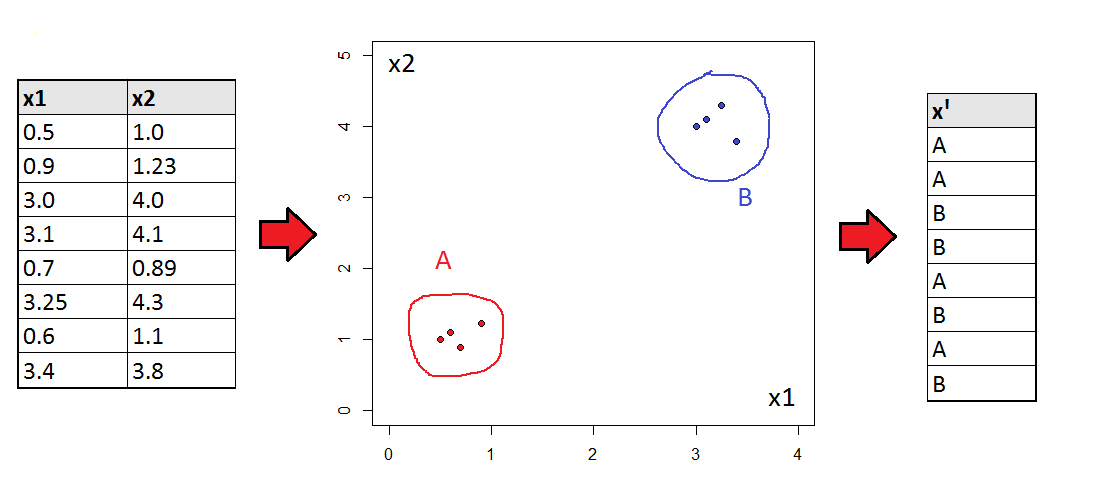
\includegraphics[height=.25\textheight]{grouping.png}
\caption{Ilustracja przestawiająca w jaki sposób grupowanie może być użyte do redukcji wymiarów. Dwuwymiarowe dane o atrybutach \emph{x\textsubscript{1}} i \emph{x\textsubscript{2}} przeniesiono na płaszczyznę i pogrupowano w dwa zbiory o etykietach \emph{A} i \emph{B}. Następnie oba atrybuty zostały zastąpione pojedynczym atrybutem \emph{x'} zawierającym etykiety przykładów. }
\label{classification:grouping}
\end{figure}

\subsection{Modele przetwarzania wstępnego}

Badając wpływ metod przetwarzania wstępnego na końcową ocenę klasyfikacji należy oddzielić obliczenia na danych trenujących od testowych. Podobnie jak ma to miejsce w przypadku klasyfikacji, metody przetwarzania wstępnego tworzą parametryczne modele bazując na danych trenujących. Przykładowo, modelem binaryzacji atrybutów jest zbiór liczb będących wartościami progów binaryzacji dla każdego atrybutu. Prowadząc badania należy pamiętać o tworzeniu modeli przetwarzania wyłącznie na danych trenujących oraz o stosowaniu tych modeli na osobnych danych testowych.

\section{Testy statystyczne}

Celem mojej pracy dyplomowej jest porównanie jakości klasyfikacji rodzin pewnych algorytmów. Aby porównanie to było wiarygodne i, aby mogło posłużyć dalszym badaniom, powinno ono używać ocen mierzonych na całej populacji, a nie na losowej próbie. Oczywistym jest, że nie dysponujemy informacjami na temat wszystkich pacjentek i możemy użyć jedynie niewielkiego zbioru danych (ok. 1000 przykładów w próbie). W związku z powyższym, aby porównanie było możliwie dokładne, wykonane zostanie z użyciem testu statystycznego.

Testem statystycznym nazywamy formułę matematyczną pozwalającą oszacować prawdopodobieństwo spełnienia pewnej hipotezy statystycznej w populacji na podstawie próby losowej z tej populacji. W przypadku mojej pracy, hipotezą zerową, którą pragniemy obalić, jest jednakowy rozkład ocen klasyfikacji dla wybranych dwóch rodzin metod. Obalenie hipotezy zerowej oznacza różnorodność rozkładów.

Testy statystyczne dzielimy na dwa rodzaje: parametryczne i nieparametryczne. Testy pierwszego rodzaju zakładają pewien ustalony rozkład danych oraz parametry tego rozkładu. Przykładami testów statystycznych są testy \emph{t-Studenta} oraz \emph{korelacja Pearsona}.

Testy nieparametryczne nie wymagają założeń odnośnie populacji, z której losowana jest próba. Dzięki mniejszej liczbie założeń do spełnienia mogą być szerzej stosowane niż testy parametryczne. Wadą testów nieparametrycznych jest mniej dokładny pomiar oraz mniejsza moc. Mocą testu nazywamy prawdopodobieństwo odrzucenia fałszywej hipotezy zerowej. W przypadku mojej pracy, testy nieparametryczne rzadziej będą wskazywać rzeczywiste różnice w rozkładach ocen pomiędzy rodzinami. Przykładami testów nieparametrycznych są test \emph{Manna-Whitneya-Wilcoxona} oraz test \emph{chi kwadrat}. 

Biorąc pod uwagę brak wiedzy a priori na temat rozkładu ocen w rodzinach metod klasyfikacji, do porównywania użyty został test nieparametryczny Manna-Whitneya-Wilcoxona. Test ten polega na policzeniu statystyki $U$, związanej z liczbą przypadków, gdzie elementy jednej z rodzin mają wartości wyższe niż elementy z drugiej rodziny. Następnie wartość $U$ porównywana jest z wartością graniczną dla ustalonych liczności rodzin oraz poziomu istotności testu. W przypadku bardzo licznych rodzin, statystyka $U$ jest zmienną losową o rozkładzie normalnym. Pozwala to w prosty sposób obliczyć \emph{p-wartość} dla danej obserwacji, a następnie porównać ją z ustalonym poziomem istotności testu.

\begin{figure}[h]
\centering
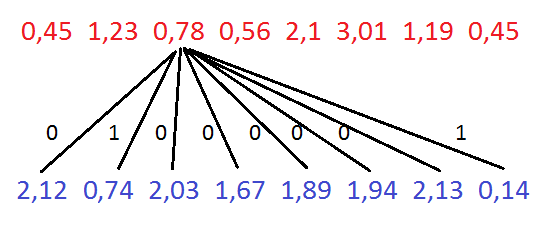
\includegraphics[height=.15\textheight]{umann.png}
\caption{Ilustracja prezentująca zasadę działania testu \emph{Manna-Whitneya-Wilcoxona} dla dwóch zbiorów danych - czerwonego i niebieskiego. Każdy element ze zbioru czerwonego porównywany jest z każdym elementem ze zbioru niebieskiego. Porównując wartości zlicza się liczbę "wygranych" dla jednego z dwóch zbiorów. }
\label{classification:umann}
\end{figure}

\section{Podsumowanie}

W tej części pracy przedstawiłem podstawowe informacje na temat przetwarzania wstępnego i klasyfikacji danych. Wyjaśniłem na czym polega klasyfikacja, jak ocenia się klasyfikatory, zwróciłem uwagę na problem nadmiernego dopasowania oraz zaprezentowałem popularne algorytmy klasyfikacji. Oprócz tego wyjaśniłem cel wstępnego przetwarzania danych oraz zaprezentowałem najpopularniejsze metody tej procedury.

Następny rozdział poświęcony jest wymaganiom systemu komputerowego służącego do porównywania algorytmów przetwarzania i klasyfikacji.

\end{document}
